\chapter{Introduction}
\label{chap:intro}
%-----------------------------------------------------------------------
The emergence of heterogeneous processor technology has enabled real-time embedded vision systems to become ubiquitous in many applications, such as robotics\cite{ZhaMenPra23}, autonomous vehicles\cite{KaiHonAma18}, and satellites\cite{PapTzioKal22}. Real-time image processing is inherently resource-intensive due to the complex algorithms that demand significant computational power and memory bandwidth. As such, optimising the performance of image processing systems requires a delicate balance between hardware capabilities, software efficiency, and algorithmic innovation to ensure timely and responsive processing. Traditionally, imaging tasks implemented on homogeneous architectures were limited in their adaptability in handling diverse sets of operations. On the contrary, the advent of heterogeneous architectures offers a flexible computing environment that combines  multiple accelerators such as CPUs, GPUs, and FPGAs, offering a choice for executing tasks according to their computational requirements.

Integrating such accelerators together poses significant challenges within design and implementation. These challenges are evident in the complexities of scheduling tasks on different hardware units, managing synchronisation, memory coherence, and addressing interconnect requirements. Additionally, the absence of standardised models for heterogeneous systems impacts the programming environment, making it challenging for developers to create cohesive applications. Lastly, performance evaluation becomes a multifaceted task, requiring a comprehensive understanding of the interactions between processing units and their contributions to overall system performance.

However, the primary challenge lies in determining the most effective approach for algorithm partitioning on heterogeneous architectures. Given that each processing architecture executes specific algorithms more efficiently than the other\cite{7577314,QasDenVis19}. In addition, navigating an environment with various tool-sets and libraries further compounds the challenge, requiring developers to carefully select and integrate the appropriate tools that align with each processor's properties. Consequently, partitioned algorithms require further hardware and algorithmic optimisations to extract maximum performance. Typically, domain-specific optimisation techniques are often overlooked limiting the full realisation of performance potential and efficiency gains.

Within the scope of the thesis, the aim is to demonstrate that leveraging heterogeneous architectures for image processing algorithms will increase performance in terms of both runtime and energy consumption. Consequently, this work introduces domain-specific optimisation techniques to further improve application efficiency. 




%Real-time embedded vision systems implemented on emerging heterogeneous processor technology have increasingly become more pervasive in applications such as robotics, autonomous vehicles and satellites. In turn, there has been an effort on developing energy-efficient image processing algorithms that can effectively exploit the underlying hardware. This is especially important for embedded vision systems that require real-time analysis where power, size and performance are the most significant constraints. Consequently, vision system designers have shifted their focus away from homogeneous hardware accelerators like CPU's or GPU's and onto heterogeneous architectures containing multiple different processing cores (\textit{Interconnected CPU+GPU+FPGA}). This way, different types of tasks can be executed by processors that are specialised in them.


\section{Motivation}
% The history of the microprocessor dates back to Fairchild Semiconductors' pivotal 1959 breakthrough in integrated circuits, setting the stage for Intel's groundbreaking release of the first commercially available microprocessor in 1971, the 4-bit Intel 4004\cite{Asp97}. Originally designed for calculators, the 4004 quickly found broader applications, marking a substantial leap in computing power with its 740 kHz clock speed. The subsequent decades witnessed a rapid evolution of microprocessors, progressing from influential 8-bit models like the Intel 8080 to 16-bit processors such as the Intel 8086 and Motorola 68000. These advancements enabled more sophisticated applications and operating systems.

% The transition from 32-bit to 64-bit architectures further expanded memory addressing capabilities, accommodating increasingly demanding applications. The early 2000s ushered in a new era with the advent of multi-core processors, revolutionising computing through parallel processing, significantly enhancing performance, and optimising efficiency. Concurrently, as microprocessors evolved, two specialised architectures emerged: Graphics Processing Units (GPUs) and Field-Programmable Gate Arrays (FPGAs). Originally designed for graphics rendering, GPUs proved adaptable for various computationally intensive tasks, thanks to their parallel processing capabilities. FPGAs, offering programmable logic and tailored hardware functionality, excelled in applications requiring low latency and high throughput, such as digital signal processing and real-time operations.


The history of the microprocessor can be traced back to 1959 when Fair-child Semiconductors made a significant breakthrough by creating the first integrated circuit. This invention revolutionised the field of electronics by laying the foundation for integrating multiple transistors and other components into a single silicon chip. In the early 1970s, Intel Corporation introduced the first commercially available microprocessor. The Intel 4004\cite{Asp97}, released in 1971, was a 4-bit processor capable of performing basic arithmetic and logical operations, with a clock speed of 740 kHz, it represented a significant leap in computing power compared to previous electronic circuits. The 4004 was primarily designed for calculators and other small-scale applications but soon found use in a wide range of devices. Many manufacturers began to contribute and innovate within the microprocessor space. In 1974, Intel released the 8080\cite{Maz07}, an 8-bit microprocessor that became highly influential. 

Continuing through the 1970s and 1980s, microprocessors advanced rapi-dly, with increasing processing power, efficiency and improved architecture capabilities. The introduction of 16-bit processors, such as the Intel 8086 and Motorola 68000, marked another significant milestone, enabling more complex applications and operating systems. In addition, ARM introduced a new architecture design which used a reduced instruction set paradigm to streamline the execution of instructions. This paved the way for the modern era of computing, with the rise of personal computers and the increasing integration of microprocessors into various devices and industries. In subsequent decades, microprocessors continued to evolve, with advancements in clock speeds, transistor densities, and architectural designs. The transition from 32-bit to 64-bit architectures expanded the memory addressing capabilities and enabled more demanding applications. Multi-core processors emerged in the early 2000s\cite{IntelCores}, revolutionising computing by enabling parallel processing and significantly improving performance and efficiency.

\begin{figure}[!tb]
\centering
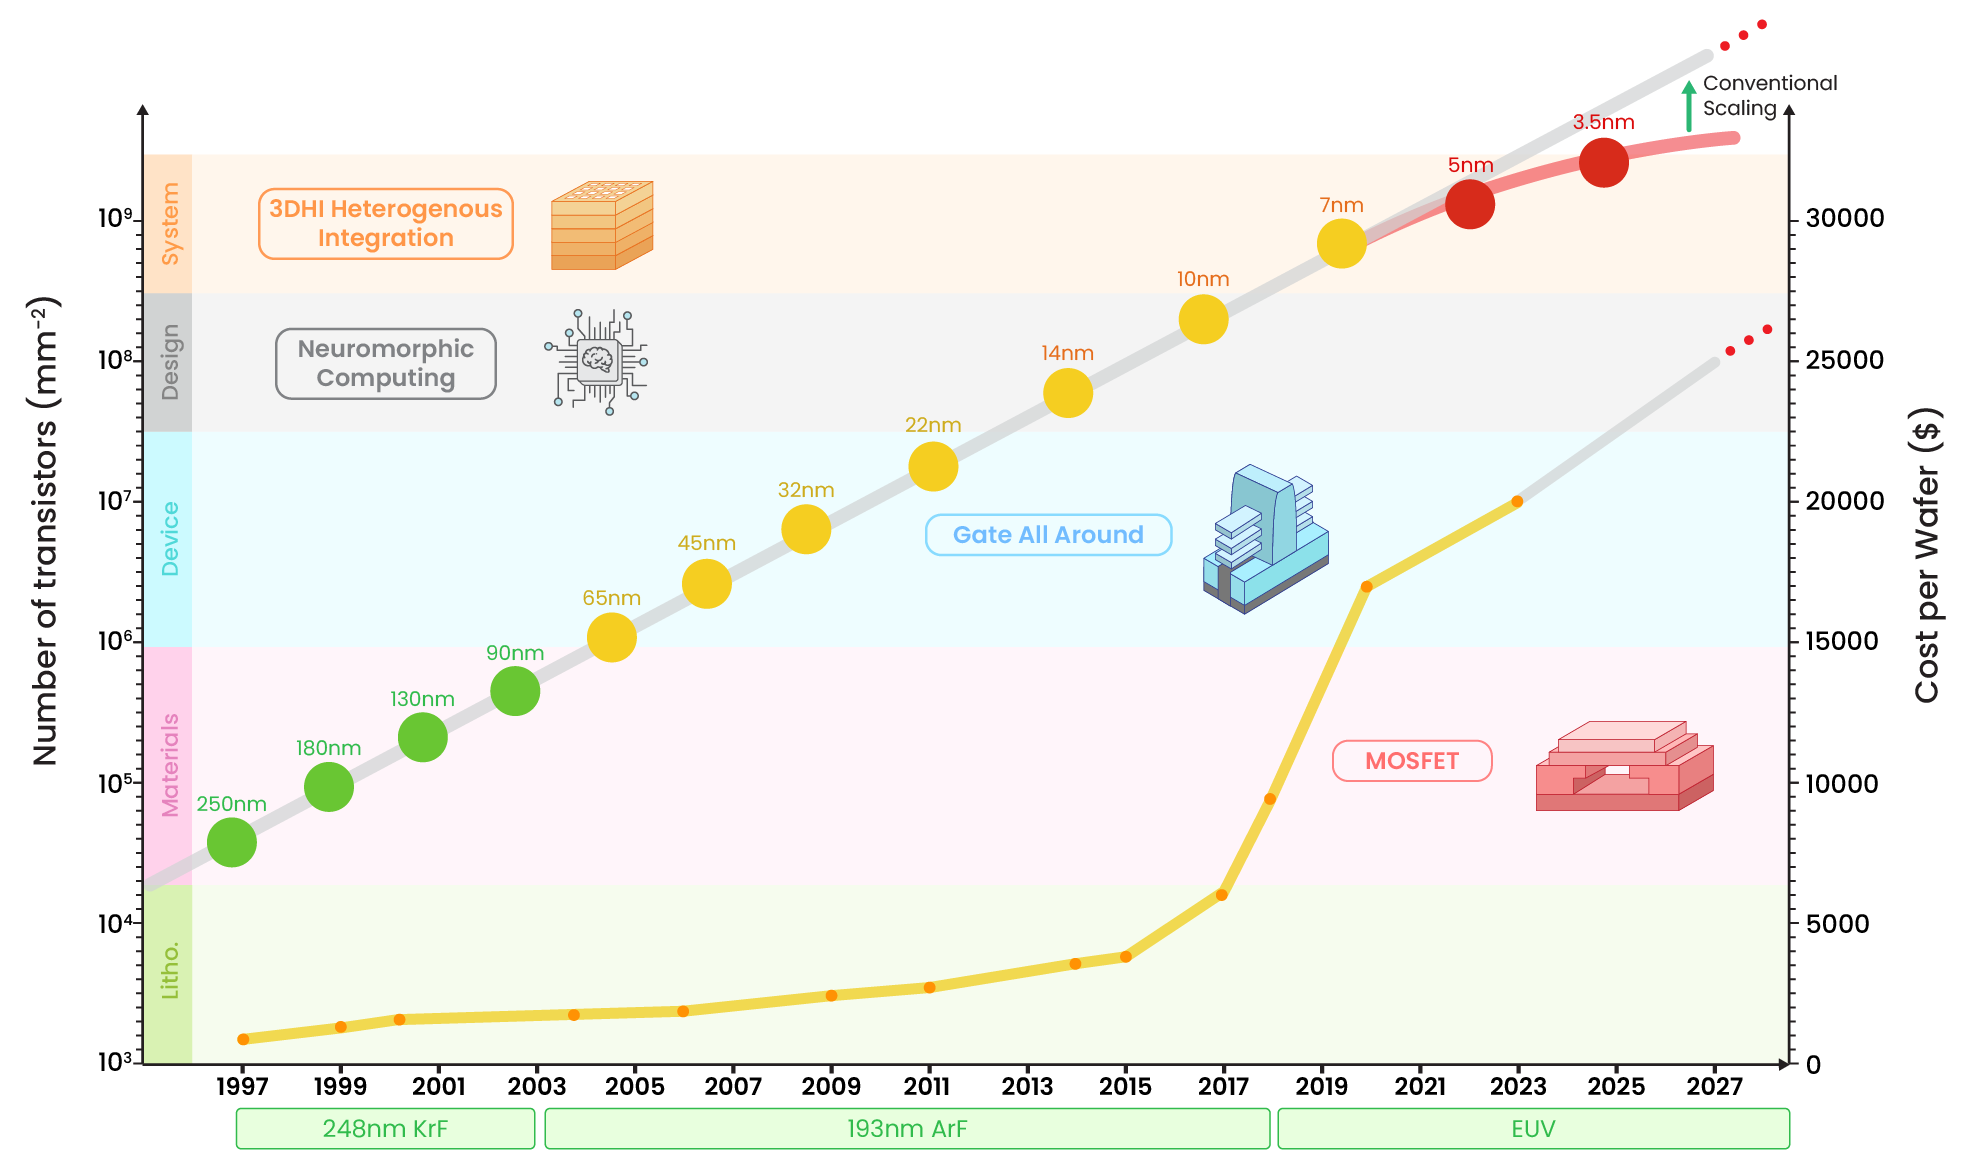
\includegraphics[width=\linewidth]{Images/transistor_chart.png}
\caption[Semiconductor Timeline]{Cost, Transistor Count \& Gate-length Technology Timeline\cite{Wafer}.}
\label{fig:Transistor}
\end{figure}  

At around the same time, as CPU processors continued to evolve, two additional specialised architectures emerged to address specific computational needs: GPUs and FPGAs. GPUs were initially designed to handle the complex computations required for rendering high-quality graphics in video games and multimedia applications. However, their parallel processing capabilities and ability to handle large amounts of data made them well-suited for other computationally intensive tasks, such as scientific simulations. On the other hand, FPGAs offer a different approach to computing. Unlike CPUs and GPUs, which are based on fixed instruction sets, FPGAs provide programmable logic that allows users to configure the hardware functionality to suit specific tasks. This flexibility enables FPGAs to be highly optimised for specific applications, such as digital signal processing, data encoding, and real-time processing. FPGAs are particularly valuable in scenarios that require low latency and high throughput, as they can be tailored to perform specific operations with exceptional efficiency.

However, in the past decade, processor architecture designs had begun to coalesce, which resulted in a convergence of approaches and a common set of design principles among different CPU manufacturers. As a result, the X86 and ARM instruction sets are the only remaining architectures used in the majority of the systems available. This shift was driven by the realisation that the exponential performance gains seen in previous years were becoming increasingly difficult to achieve due to physical limitations and power constraints, reflected in \Fig{Transistor}.

% \begin{figure}[!ht]
% \centering
% 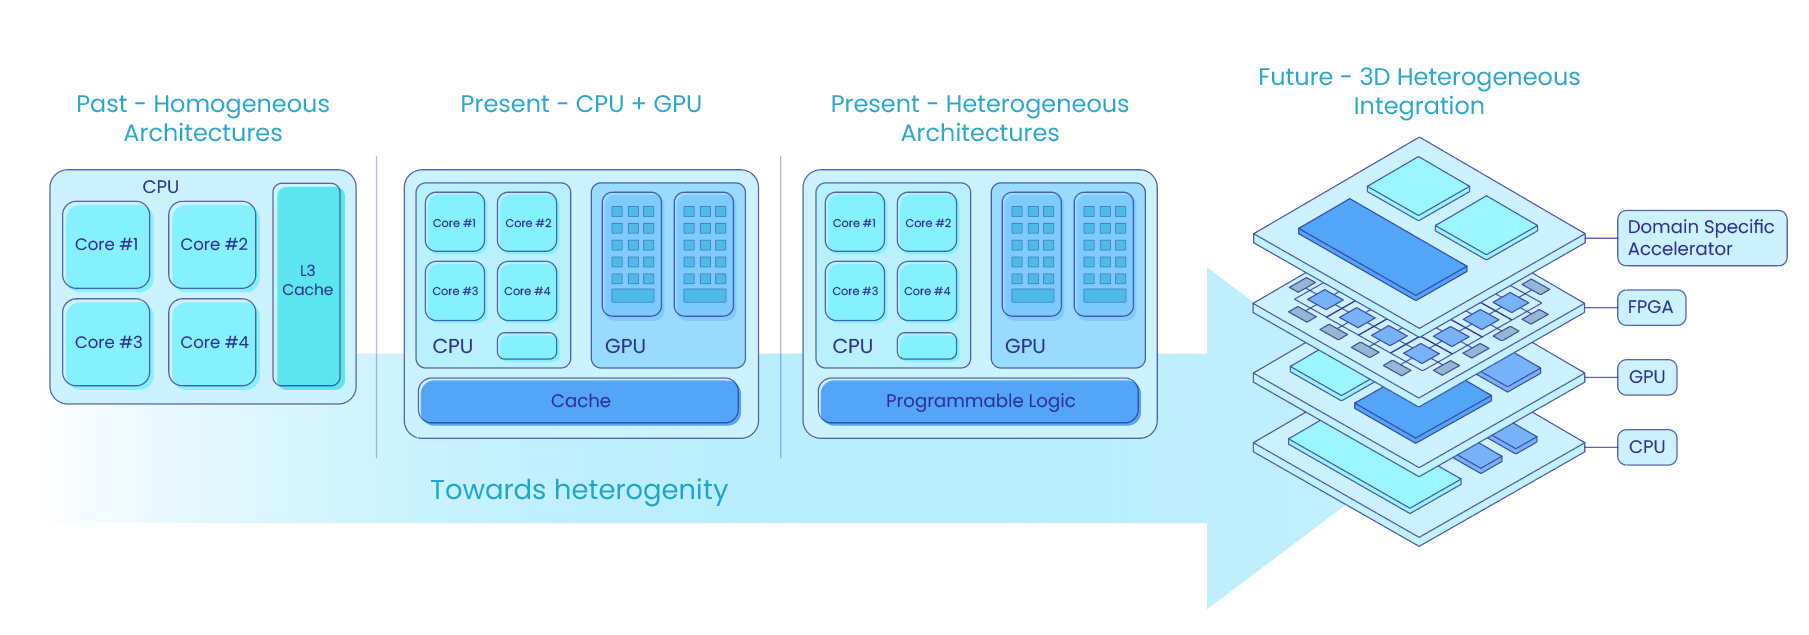
\includegraphics[width=\linewidth]{Images/TowardHeterogeniety.png}
% \caption[Processing Architecture Timeline]{Moving from Homogeneous Processing Architectures Towards Heterogeneity by Combining Various Specialised Accelerators using 3D Stacking Process Technology.}
% \label{fig:TowardHeterogeniety}
% \end{figure} 

The recent emergence of deep learning has reignited the pursuit of specialised computing units, which has fragmented the ecosystem. Developers have started exploring the potential of domain-specific accelerators such as TPUs or NPUs to meet specific computational needs. As a result, the processor landscape has become increasingly diverse again, with different manufacturers pursuing their unique architectural approaches. The growing set of domain-specific accelerators has driven designers to adopt newer and innovative approaches involving heterogeneity. A chiplet-based approach has emerged as a promising paradigm by disaggregating specialised processing units and integrating them into a cohesive interconnected circuit. Each chiplet serves a specific function, leveraging modularity and specialisation to enhance performance, scalability, and customisation. In addition, new packaging methods are utilised to integrate chiplets together, ranging from 2.5D-IC silicon interposers to 3D stacking. Nevertheless, with the deployment of diverse and heterogeneous architectures, a crucial challenge arises in the form of designing algorithms capable of effectively harnessing the capabilities offered by these novel architectural frameworks. This necessitates the development of algorithmic approaches that can optimise performance, exploit parallelism, and efficiently use the unique features and resources provided by these heterogeneous systems.


\begin{figure}[tb]
\centering
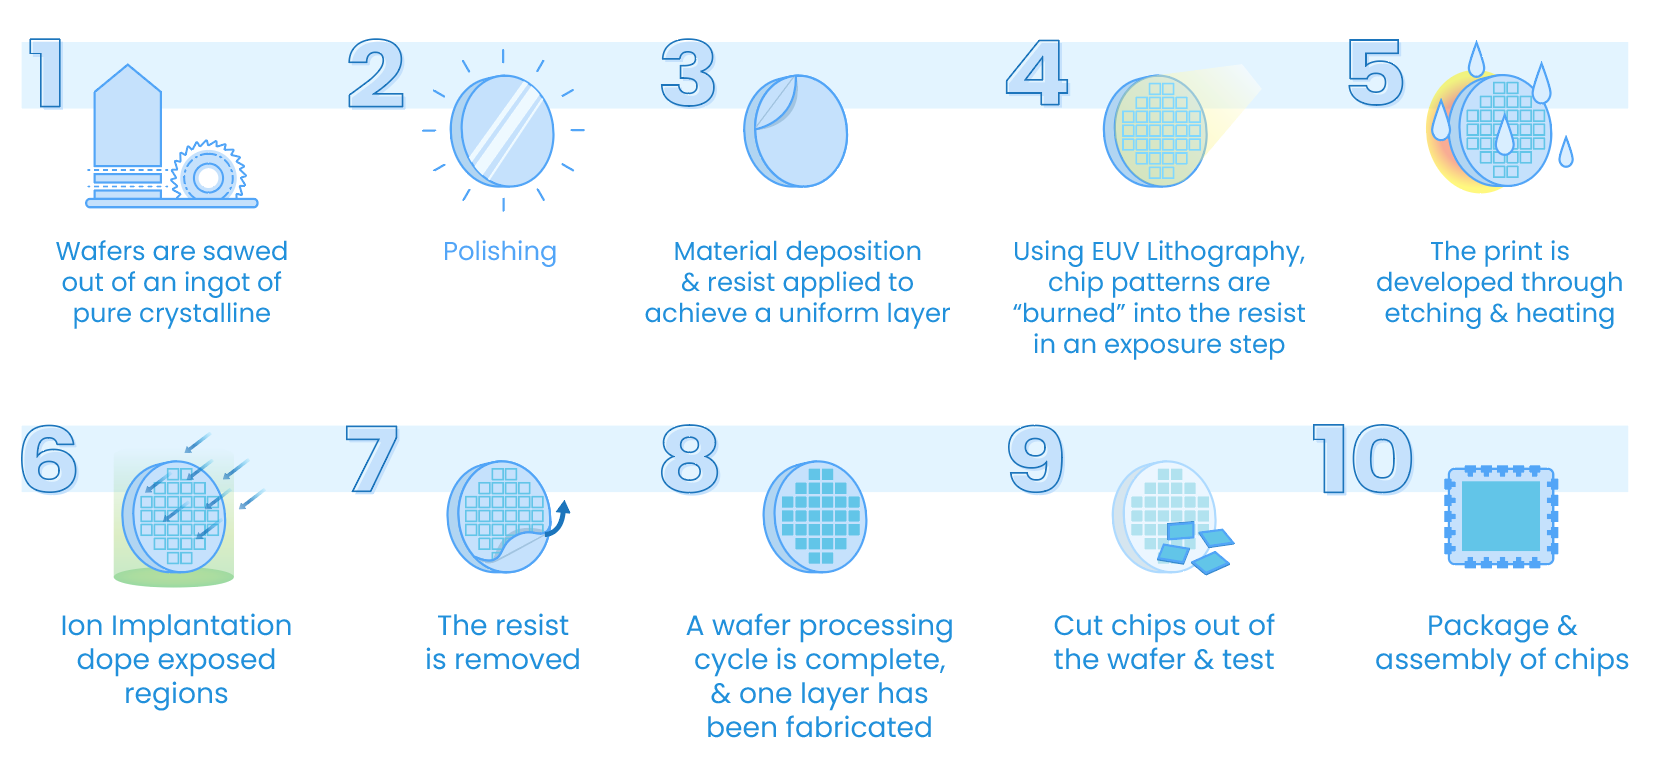
\includegraphics[width=\linewidth]{Images/image.png}
\caption[Wafer Fabrication]{Wafer Fabrication Process Steps to Develop Microprocessors.}
\label{fig:fabrication}
\end{figure} 

% \subsubsection{Wafer Fabrication}
Wafer fabrication, involves a series of steps to transform a silicon wafer into an integrated circuit shown in \Fig{fabrication}, including wafer preparation, photolithography, etching, layer deposition, and testing for functionality and quality. The pursuit of smaller transistor sizes, driven by demands for enhanced memory capacity and processing capabilities, has led to heavy investment in novel lithography technologies. However, the doubling of transistor densities every two years, as predicted by Moore's Law, has started to deviate due to technological limitations and economic costs. Shrinking transistors face challenges from the limitations of lithography wavelengths and the increasing complexity of manufacturing processes, leading to lower yields and higher costs. The production of larger silicon wafers has been debated, with the industry transitioning from small diameters in the 1960s to 300mm wafers as the standard by the early 1990s. While larger wafers offer cost and yield benefits, transitioning requires equipment redesign and cost-effectiveness considerations.
% Wafer fabrication, or semiconductor manufacturing, involves a series of steps shown in \Fig{fabrication} to transform a silicon wafer into an integrated circuit. The process includes wafer preparation, photolithography to define the circuit pattern, etching to remove material, deposition of layers, and additional steps like planarisation and implantation. Tests are conducted to assess functionality and quality. The wafer is then packaged, and tested again before integration into electronic devices. In the field of processor fabrication, the pursuit towards achieving smaller transistor sizes stems from the demands imposed by modern applications in terms of enhanced memory capacity and processing capabilities. 

% These requirements have pushed semiconductor manufacturers to invest heavily in novel lithography technologies and tools. The transistor densities in the last two decades have started to deviate from the projected doubling every two years. Moore's Law has been a guiding principle for the semiconductor industry since its inception, predicting that the number of transistors that can be placed on an integrated circuit doubles approximately every two years. However, there is growing evidence that this trend is beginning to taper off. The two primary reasons for this are 1) technological limitations and 2) economic cost, which fundamentally dictate the production of integrated circuits. In the context of technology, as transistors shrink to ever smaller sizes, the wavelengths of light used in lithography become a significant limiting factor. Moreover, the increasing complexity of the manufacturing process is another significant challenge faced by semiconductor fabrication. As gate lengths continue to decrease, the number of steps required for chip fabrication increases, leading to a more costly, laborious and time-consuming manufacturing process. This complexity raises the likelihood of defects during manufacturing, resulting in lower yields and higher costs.

% The economics driving the production of larger silicon wafers has been a divisive issue in the past decade. The size of silicon wafers used in device fabrication evolved over time. Initially, in the 1960s, manufacturers used wafers that were only a few millimetres in diameter, typically between 25mm and 75mm. In the 1980s, the industry transitioned to larger 150mm wafers, and by the early 1990s and onwards, 300mm wafers had become the standard. Historically, moving to larger wafers was an essential path for foundries by enabling the production of more dice per wafer while using the same number of process steps resulted in overall cost and yield benefits. However, switching wafer dimensions requires fabrication equipment to be redesigned since the tools form a pipeline which in turn leads to requiring all vendors to accommodate the change. In any case, wafer-size transitions will not become a reality until they can be made more cost-effective. 

In summary, recent years have brought about major changes in the semiconductor industry, driven by the demand from resource intensive algorithms such as image processing and higher wafer fabrication cost. As a result, heterogeneous architectures serve as a potential to increase system performance further. However, understanding how to efficiently partition algorithms on each accelerator and identifying domain-specific optimisation trade-offs remain key challenges in maximising the potential of these architectures.

\newpage

\section{Research Objectives}
This thesis aims to conduct research on partitioning and optimising image processing algorithms on heterogeneous architectures to unlock the full energy and runtime performance. This research encompasses a wide range of multidisciplinary domains (\eg hardware (CPU/GPU/FPGA), compilers, schedulers, optimisations and programming languages). Therefore, the focus is refined to three primary objectives in this thesis, which are listed in detail below:  

\begin{enumerate}
    \item Understanding the properties of image processing algorithms and hardware to determine the suitability in order to map operations to the most efficient hardware to increase performance. In addition, exploring optimised tool-sets and libraries in terms of programmability and performance. The goal of this objective is to develop a comprehensive micro/macro bench-marking framework which distils algorithms into their principle operations and gives heuristics towards mapping the operations to correct architecture. Additionally, providing various metrics to evaluate and compare each accelerator. This work enables the partitioning of algorithms on heterogeneous architectures, as realised in later chapters
    
    \item Investigating domains-specific optimisation techniques which leads to better performance on hardware by exploiting inherent characteristics and structures in the image domain. These optimisations are applied in various combinations to determine the trade-offs in runtime, energy and accuracy metrics. The outcomes of this research enable understanding the efficiency of various hardware-agnostic optimisation methods found within the image processing domain.

    \item Development of a comprehensive heterogeneous platform capable of executing image processing operations across all processing units while efficiently scheduling data for optimal performance. This includes designing and developing two complete heterogeneous platforms for high and low-power applications. Furthermore, using novel layer-wise/stage partitioning techniques on convolutional neural networks and feature extraction algorithms to execute on the most suitable accelerator within the heterogeneous platform. The goal of the objective is to uncover the advantages of heterogeneous architectures in image processing and document their performance gains over single-device solutions.

    
    \end{enumerate}



%his thesis aims to establish a systematic benchmark framework to partition and implement image processing algorithms heterogeneous platforms by identifying algorithmic and processing unit characteristics to suggest their suitability. Furthermore, domain-specific optimisations are explored and its impacts are analysed on each accelerators to understand the performance trade-offs. Finally, popular deep learning vision architectures are implemented and evaluated on two constructed heterogeneous platforms targeting high and low energy consumption requirements.




%For example, once Lithography vendors switch, You also need plasma etchers, CMP machines, diffusion furnaces, metrology, and more. 
%Every piece of equipment needs to be available in \textit{$X mm$} form before a manufacturer can build the first \textit{$X mm$} fab. Therefore, both foundries and equipment manufacturers have been locked in a disagreement on upfronting the cost of transitioning from 300mm to 450mm silicon wafers and determining how substantial initial investment would be recovered. 

% In summary, recent years have brought about significant changes in the
% semiconductor industry, driven by the demand from resource intensive al-
% gorithms such as image processing and higher wafer fabrication cost. As a
% result, heterogeneous architectures serve as a potential to increase system
% performance further. However, understanding how to efficiently partition
% algorithms on each accelerator and identifying domain-specific optimisation
% trade-offs remain key challenges in maximising the potential of these archi-
% tectures. The thesis aims to



% The history of the microprocessor can be traced back to 1959 when Fair-child Semiconductors made a significant breakthrough by creating the first integrated circuit. This invention revolutionised the field of electronics by laying the foundation for integrating multiple transistors and other components into a single silicon chip. In the early 1970s, Intel Corporation introduced the first commercially available microprocessor. The Intel 4004\cite{Asp97}, released in 1971, was a 4-bit processor capable of performing basic arithmetic and logical operations, with a clock speed of 740 kHz, it represented a significant leap in computing power compared to previous electronic circuits. The 4004 was primarily designed for calculators and other small-scale applications but soon found use in a wide range of devices. Many manufacturers began to contribute and innovate within the microprocessor space. In 1974, Intel released the 8080\cite{Maz07}, an 8-bit microprocessor that became highly influential. 

% Continuing through the 1970s and 1980s, microprocessors advanced rapi-dly, with increasing processing power, efficiency and improved architecture capabilities. The introduction of 16-bit processors, such as the Intel 8086 and Motorola 68000, marked another significant milestone, enabling more complex applications and operating systems. In addition, ARM introduced a new architecture design which used a reduced instruction set paradigm to streamline the execution of instructions. This paved the way for the modern era of computing, with the rise of personal computers and the increasing integration of microprocessors into various devices and industries. In subsequent decades, microprocessors continued to evolve, with advancements in clock speeds, transistor densities, and architectural designs. The transition from 32-bit to 64-bit architectures expanded the memory addressing capabilities and enabled more demanding applications. Multi-core processors emerged in the early 2000s, revolutionising computing by enabling parallel processing and significantly improving performance and efficiency.

% At around the same time, as CPU processors continued to evolve, two additional specialised architectures emerged to address specific computational needs: GPUs and FPGAs. GPUs were initially designed to handle the complex computations required for rendering high-quality graphics in video games and multimedia applications. However, their parallel processing capabilities and ability to handle large amounts of data made them well-suited for other computationally intensive tasks, such as scientific simulations. On the other hand, FPGAs offer a different approach to computing. Unlike CPUs and GPUs, which are based on fixed instruction sets, FPGAs provide programmable logic that allows users to configure the hardware functionality to suit specific tasks. This flexibility enables FPGAs to be highly optimised for specific applications, such as digital signal processing, data encoding, and real-time processing. FPGAs are particularly valuable in scenarios that require low latency and high throughput, as they can be tailored to perform specific operations with exceptional efficiency.

% \begin{figure}[!tb]
% \centering
% 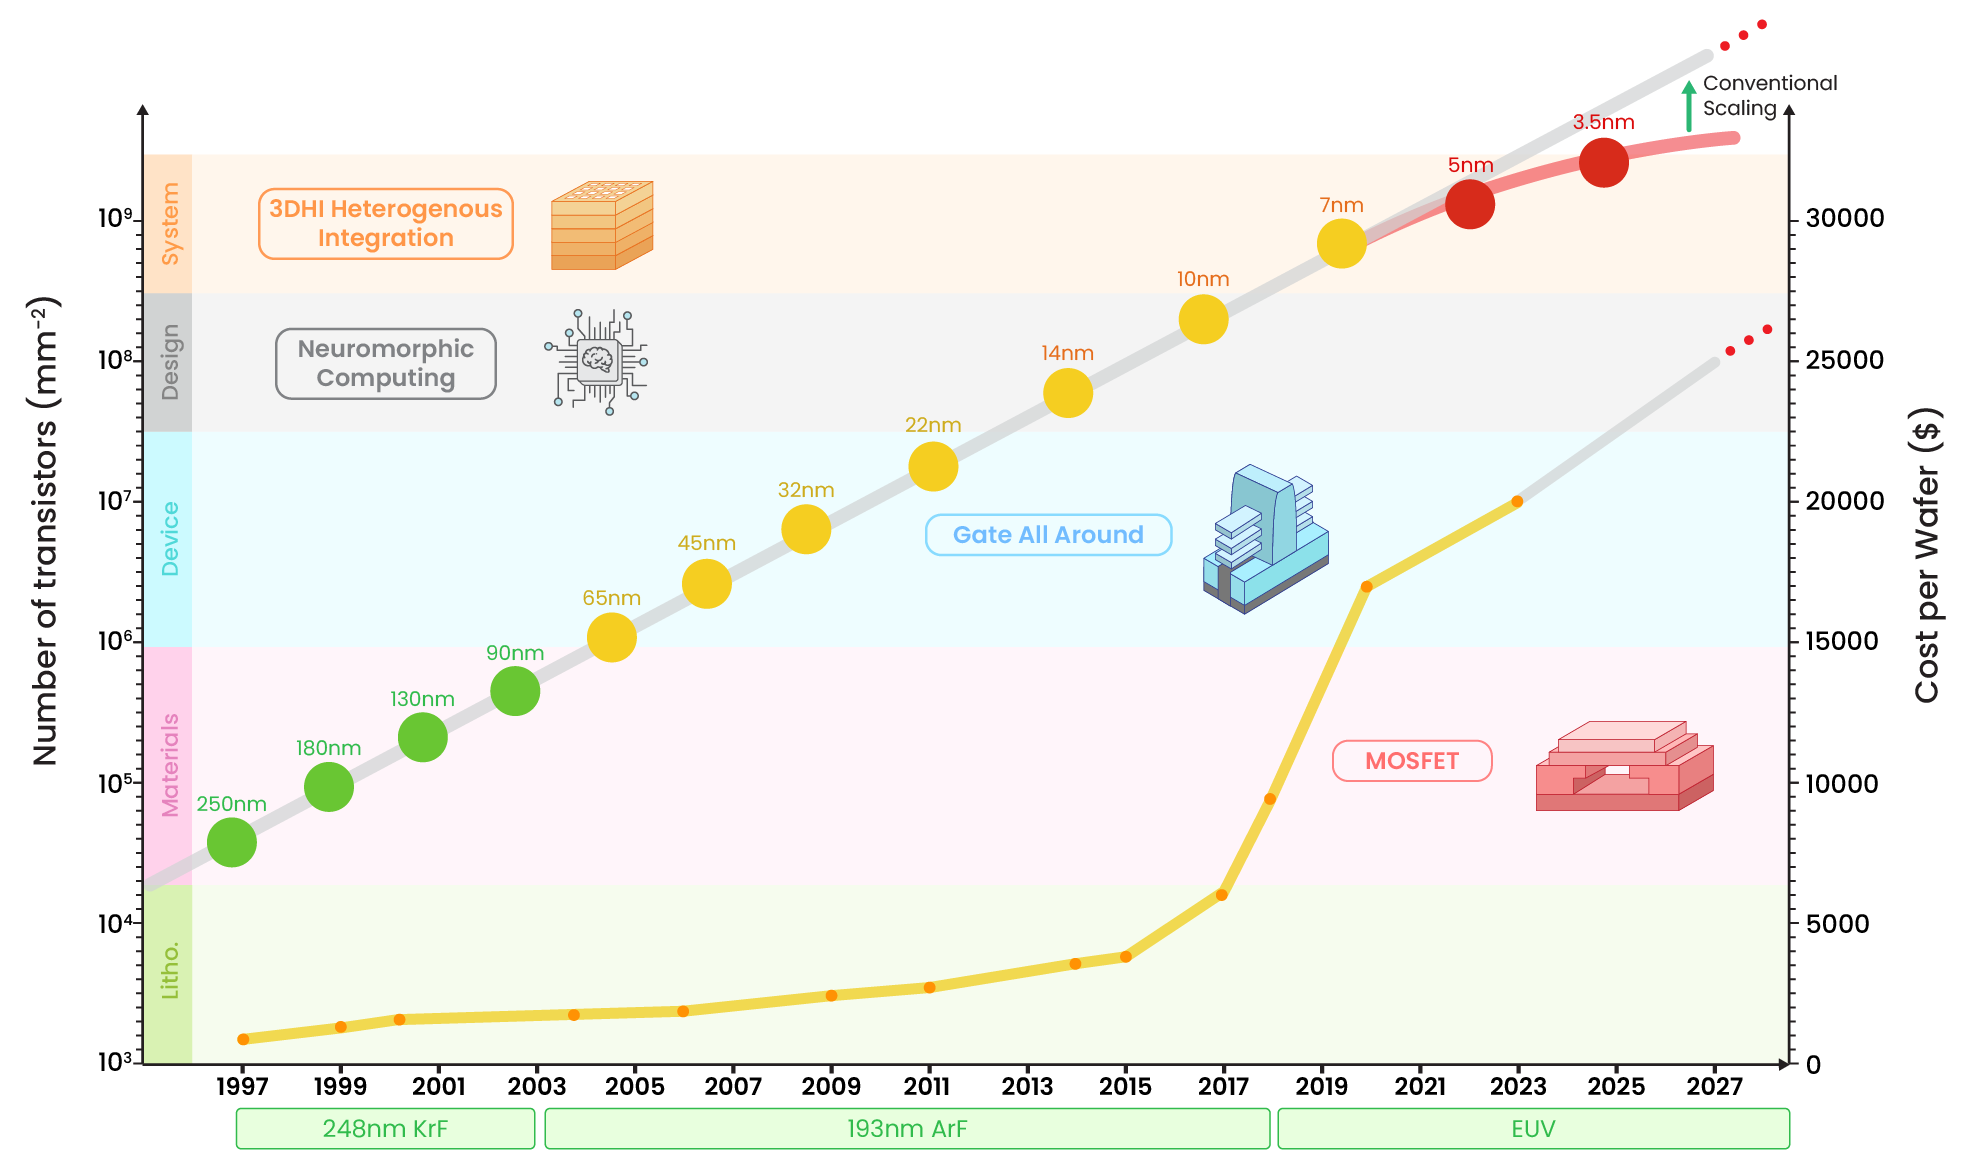
\includegraphics[width=\linewidth]{Images/transistor_chart.png}
% \caption[Semiconductor Timeline]{Cost, Transistor Count \& Gate-length Technology Timeline\cite{Wafer}.}
% \label{fig:Transistor}
% \end{figure} 

% However, in the past decade, processor architecture designs had begun to coalesce, which resulted in a convergence of approaches and a common set of design principles among different CPU manufacturers. As a result, the X86 and ARM instruction sets are the only remaining architectures used in the majority of the systems available. This shift was driven by the realisation that the exponential performance gains seen in previous years were becoming increasingly difficult to achieve due to physical limitations and power constraints, reflected in \Fig{Transistor}.

% \begin{figure}[!t]
% \centering
% 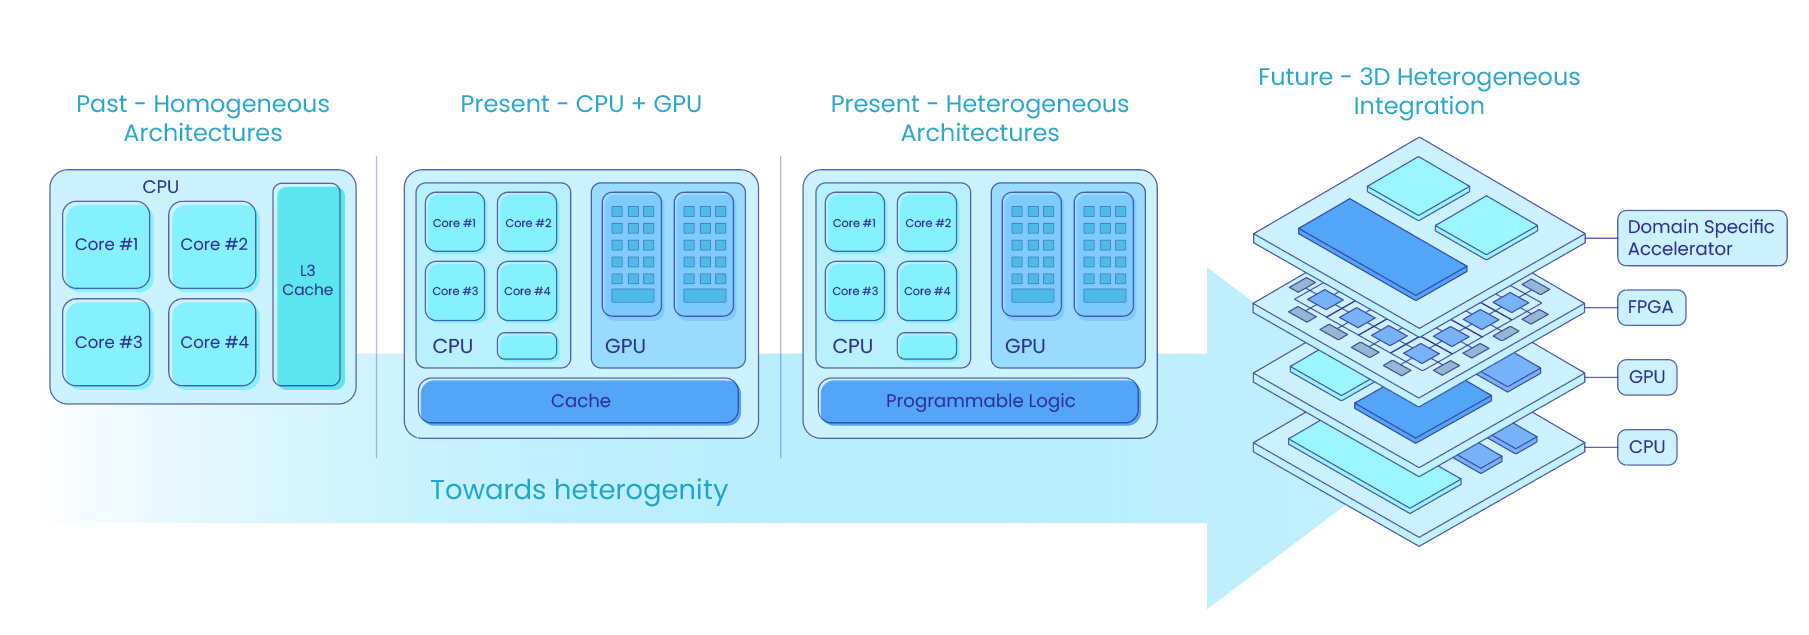
\includegraphics[width=\linewidth]{Images/TowardHeterogeniety.png}
% \caption[Processing Architecture Timeline]{Moving from Homogeneous Processing Architectures Towards Heterogeneity by Combining Various Specialised Accelerators using 3D Stacking Process Technology.}
% \label{fig:TowardHeterogeniety}
% \end{figure} 

% Real-time image processing has witnessed a remarkable surge in importance and applicability in the last decade, propelled by advances in autonom-ous systems, augmented reality (AR), and robotics. Real-time image processing is inherently resource-intensive due to the complex algorithms that demand significant computational power and memory bandwidth. As such, optimising the performance of image processing systems requires a delicate balance between hardware capabilities, software efficiency, and algorithmic innovation to ensure timely and responsive processing. Furthermore, The emergence of deep learning has reignited the pursuit of specialised computing units, which has fragmented the ecosystem. Developers have started exploring the potential of domain-specific accelerators such as TPUs or NPUs to meet specific computational needs. As a result, the processor landscape has become increasingly diverse again, with different manufacturers pursuing their unique architectural approaches. The growing set of domain-specific accelerators has driven designers to adopt newer and innovative approaches involving heterogeneity, observed in \Fig{TowardHeterogeniety}. The chiplet-based approach has emerged as a promising paradigm by disaggregating specialised processing units and integrating them into a cohesive interconnected circuit. Each chiplet serves a specific function, leveraging modularity and specialisation to enhance performance, scalability, and customisation. In addition, new packaging methods are utilised to integrate chiplets together, ranging from 2.5D-IC silicon interposers to 3D stacking. Nevertheless, with the deployment of diverse and heterogeneous architectures, a crucial challenge arises in the form of designing algorithms capable of effectively harnessing the capabilities offered by these novel architectural frameworks. This necessitates the development of algorithmic approaches that can optimise performance, exploit parallelism, and efficiently use the unique features and resources provided by these heterogeneous systems.





% \section{Semiconductor Technology}


% \begin{figure}[!h]
% \centering
% 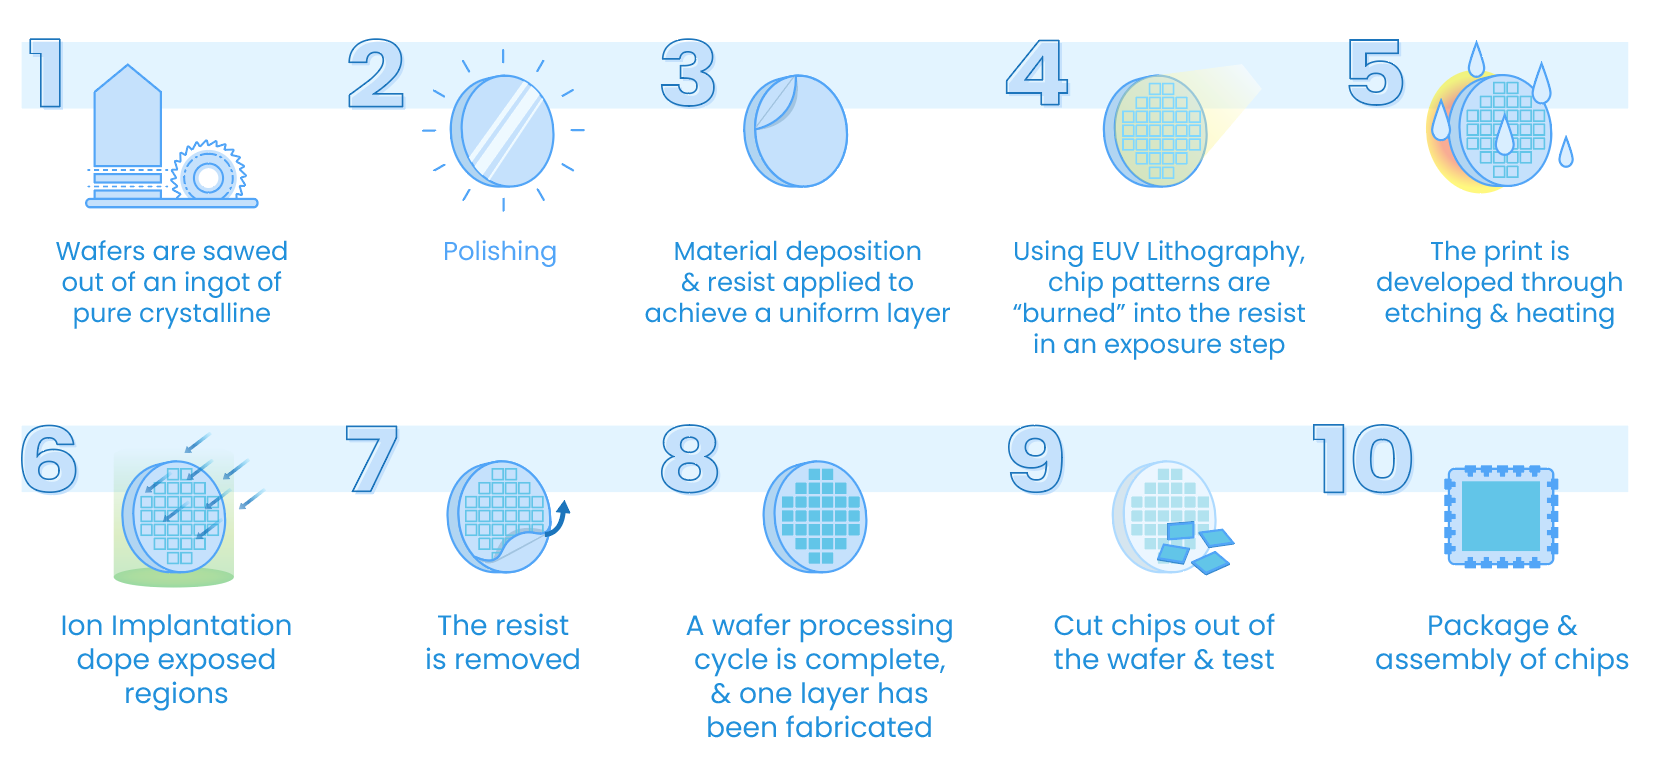
\includegraphics[width=\linewidth]{Images/image.png}
% \caption[Wafer Fabrication]{Wafer Fabrication Process Steps to Develop Microprocessors.}
% \label{fig:fabrication}
% \end{figure} 

% Wafer fabrication, or semiconductor manufacturing, involves a series of steps shown in \Fig{fabrication} to transform a silicon wafer into an integrated circuit. The process includes wafer preparation, photolithography to define the circuit pattern, etching to remove material, deposition of layers, and additional steps like planarisation and implantation. Tests are conducted to assess functionality and quality. The wafer is then packaged, and tested again before integration into electronic devices. In the field of processor fabrication, the pursuit towards achieving smaller transistor sizes stems from the demands imposed by modern applications in terms of enhanced memory capacity and processing capabilities. 

% These requirements have pushed semiconductor manufacturers to invest heavily in novel lithography technologies and tools. The transistor densities in the last two decades have started to deviate from the projected doubling every two years. Moore's Law has been a guiding principle for the semiconductor industry since its inception, predicting that the number of transistors that can be placed on an integrated circuit doubles approximately every two years. However, there is growing evidence that this trend is beginning to taper off. The two primary reasons for this are 1) technological limitations and 2) economic cost, which fundamentally dictate the production of integrated circuits. In the context of technology, as transistors shrink to ever smaller sizes, the wavelengths of light used in lithography become a significant limiting factor. Moreover, the increasing complexity of the manufacturing process is another significant challenge faced by semiconductor fabrication. As gate lengths continue to decrease, the number of steps required for chip fabrication increases, leading to a more costly, laborious and time-consuming manufacturing process. This complexity raises the likelihood of defects during manufacturing, resulting in lower yields and higher costs.

% The economics driving the production of larger silicon wafers has been a divisive issue in the past decade. The size of silicon wafers used in device fabrication evolved over time. Initially, in the 1960s, manufacturers used wafers that were only a few millimetres in diameter, typically between 25mm and 75mm. In the 1980s, the industry transitioned to larger 150mm wafers, and by the early 1990s and onwards, 300mm wafers had become the standard. Historically, moving to larger wafers was an essential path for foundries by enabling the production of more dice per wafer while using the same number of process steps resulted in overall cost and yield benefits. However, switching wafer dimensions requires fabrication equipment to be redesigned since the tools form a pipeline which in turn leads to requiring all vendors to accommodate the change. %For example, once Lithography vendors switch, You also need plasma etchers, CMP machines, diffusion furnaces, metrology, and more. 
% Every piece of equipment needs to be available in \textit{$X mm$} form before a manufacturer can build the first \textit{$X mm$} fab. Therefore, both foundries and equipment manufacturers have been locked in a disagreement on upfronting the cost of transitioning from 300mm to 450mm silicon wafers and determining how substantial initial investment would be recovered. In any case, wafer-size transitions will not become a reality until they can be made more cost-effective. 

% In summary, recent years have brought about significant changes in the semiconductor industry, driven by the demand from resource intensive algorithms such as image processing and higher wafer fabrication cost. As a result, heterogeneous architectures serve as a potential to increase system performance further. However, understanding how to efficiently partition algorithms on each accelerator and identifying domain-specific optimisation trade-offs remain key challenges in maximising the potential of these architectures.


%Real-time embedded vision systems implemented on emerging heterogeneous processor technology have increasingly become more pervasive in applications such as robotics, autonomous vehicles and satellites. In turn, there has been an effort on developing energy-efficient image processing algorithms that can effectively exploit the underlying hardware. This is especially important for embedded vision systems that require real-time analysis where power, size and performance are the most significant constraints. Consequently, vision system designers have shifted their focus away from homogeneous hardware accelerators like CPU's or GPU's and onto heterogeneous architectures containing multiple different processing cores (\textit{Interconnected CPU+GPU+FPGA}). This way, different types of tasks can be executed by processors that are specialised in them.

\section{Thesis Outline}
The rest of this thesis is organised as follows:

\textbf{Chapter 2} presents a technical background on the devices, tools and software deployed in end to end imaging pipelines. This encompasses types of imaging sensors, interfaces, hardware architectures for image processing, high-level synthesis tools and Domain Specific Languages, followed by general discussions of their advantages and drawbacks within the image processing domain.\par

\textbf{Chapter 3} critically discusses the state-of-the-art in current literature on optimisations and architectures, which includes HLS/DSL tools, micro/macro benchmarking frameworks and methodologies. Furthermore, an analysis of heterogeneous hardware and their performance in image and domain-specific optimisations.   

\textbf{Chapter 4} presents a novel framework methodology \textit{HArBoUR}, for heterogeneous architectures which deconstructs image processing pipelines into their fundamental operations and evaluates their performance on hardware platforms, including CPUs, GPUs, and FPGAs. The methodology extends its evaluation to include various hardware based performance metrics, enabling a finer-grained analysis of each architecture's capabilities.

\textbf{Chapter 5} presents the proposition of domain-specific optimisations for various imaging and deep-learning algorithms. Each optimisation strategy is applied individually and in combination, and their effectiveness is validated using runtime, accuracy and energy consumption metrics.

\textbf{Chapter 6} proposes two algorithm types and their implementations on heterogeneous architectures, two convolution neural networks and one feature extraction algorithm. The accuracy, energy consumption and runtimes are recorded and compared to their discrete counterparts.

\textbf{Chapter 7} concludes this thesis by summarising the research outcomes, i.e., analysis, proposed benchmarking framework and optimisation strategies on heterogeneous algorithms. Novel contributions are highlighted here along with suggestions on new ideas for future research in this domain.

\section{Publications}

\subsection*{Journals}
\textbf{Ali, T.}, Bhowmik, D. \& Nicol, R. Domain-Specific Optimisations for Image Processing on FPGAs. Journal of Signal Process Systems (2023). \newline
\url{https://doi.org/10.1007/s11265-023-01888-2}

\subsection*{Reports}
M, Bane, O, Brown, \textbf{T, Ali}, D, Bhowmik, J, Quinn, D, Stansby. ENERGETIC (ENergy aware hEteRoGenEous compuTIng at sCale). \newline
\url{https://doi.org/10.23634/MMU.00631226}

\subsection*{Under Preparation}
\textbf{Ali, T.}, Bhowmik, D. \& Nicol, R. A Benchmarking Framework for Imaging Algorithms on Heterogeneous Architectures. 

\begin{flushleft}
\textbf{Ali, T.}, Bhowmik, D. \& Nicol, R. Energy Aware CNN Deployment on Heterogeneous Architectures.
\end{flushleft}
